\documentclass[12pt, letterpaper, twoside]{article}
\usepackage{amsmath, amssymb}
\usepackage{physics}
\usepackage{mathtools}
\usepackage{hyperref}
\usepackage{lipsum}
\usepackage{xcolor}
\hypersetup{
    colorlinks,
    linkcolor={blue},
    citecolor={blue},
    urlcolor={blue}
}

\usepackage[letterpaper,
            margin=0.8in]{geometry}

\title{Astro 507; Problem Set 1}
\author{\textbf{Tom Wagg}}
\date{January 20, 2022}

\newcommand{\question}[1]{{\noindent \it #1}}
\newcommand{\answer}[1]{
    \par\noindent\rule{\textwidth}{0.4pt}#1\vspace{0.5cm}
}
\newcommand{\todo}[1]{{\color{red}\begin{center}TODO: #1\end{center}}}

% custom function for adding units
\makeatletter
\newcommand{\unit}[1]{%
    \,\mathrm{#1}\checknextarg}
\newcommand{\checknextarg}{\@ifnextchar\bgroup{\gobblenextarg}{}}
\newcommand{\gobblenextarg}[1]{\,\mathrm{#1}\@ifnextchar\bgroup{\gobblenextarg}{}}
\makeatother

\newcommand{\avg}[1]{\left\langle #1 \right\rangle}
\allowdisplaybreaks

\begin{document}

\maketitle

\noindent\textbf{Links for your convenience}\\
The implementation of my simulation can be found here: \url{https://github.com/TomWagg/thermo_winter22/blob/tom/pset1}. The simulation code specifically is in \texttt{simulator.py}. All code for reproducing figures can be found in this folder under files called \texttt{problem\_x.py}, where \texttt{x} is the problem number. Additionally, full size figure files are in the \texttt{figures} directory.\\

\question{1a. \textbf{Code Summary}}
\answer{
    I initially wrote this simulation in a more object-oriented way but found that it was a tad slow and so switched to keeping track of everything in arrays and vectorising the code. The \texttt{Simulation} class handles pretty much everything and you can input the particle/box details in this Class.
    
    I use cgs units for my variables: sizes are in centimetres, masses are in grams, times in seconds, and energies in ergs. I visualise the code using \texttt{tkinter} which a group of us set up with a lot of help from David! This can be toggled on or off by using the \texttt{visualise} parameter in the initialisation function of the class.
    
    I determine whether a collision has occurred by checking whether these two conditions hold
    \begin{align}
        \norm{\vb{x_1} - \vb{x_2}} &<= r_1 + r_2 \\
        \vb{v_1} \cdot \vb{v_2} &< 0
    \end{align}
    where $\vb{x}$ is the position of a particle, $r$ is the radius of a particle, $\vb{v}$ is the velocity of a particle and the subscript correspond to the different particles. These conditions ensure that the particles are in contact and moving towards one another.
    
    For resolving particle collisions I solve these equations (which I got from \href{https://en.wikipedia.org/wiki/Elastic_collision\#Two-dimensional_collision_with_two_moving_objects}{here})
    \begin{align}
        \mathbf{v}_{1}^{\prime} &= \mathbf{v}_{1}-\frac{2 m_{2}}{m_{1}+m_{2}} \frac{\left\langle\mathbf{v}_{1}-\mathbf{v}_{2}, \mathbf{x}_{1}-\mathbf{x}_{2}\right\rangle}{\left\|\mathbf{x}_{1}-\mathbf{x}_{2}\right\|^{2}}\left(\mathbf{x}_{1}-\mathbf{x}_{2}\right) \\
        \mathbf{v}_{2}^{\prime} &= \mathbf{v}_{2}-\frac{2 m_{1}}{m_{1}+m_{2}} \frac{\left\langle\mathbf{v}_{2}-\mathbf{v}_{1}, \mathbf{x}_{2}-\mathbf{x}_{1}\right\rangle}{\left\|\mathbf{x}_{2}-\mathbf{x}_{1}\right\|^{2}}\left(\mathbf{x}_{2}-\mathbf{x}_{1}\right)
    \end{align}
    These equations essentially redistribute the velocity along the contact angle based on the initial velocities of each particle and their masses, $m$.
    
    Finally, for wall collisions, I check whether a particle is within a radius of one of the edges of the box. If this is the case, I reflect the velocity component that is perpendicular to the wall.
}

\pagebreak

\question{1b. \textbf{Snapshot Plots}}
\answer{
    The initial and final distributions of particles are shown in Figure~\ref{fig:1b}.
    \begin{figure}[htbp]
        \centering
        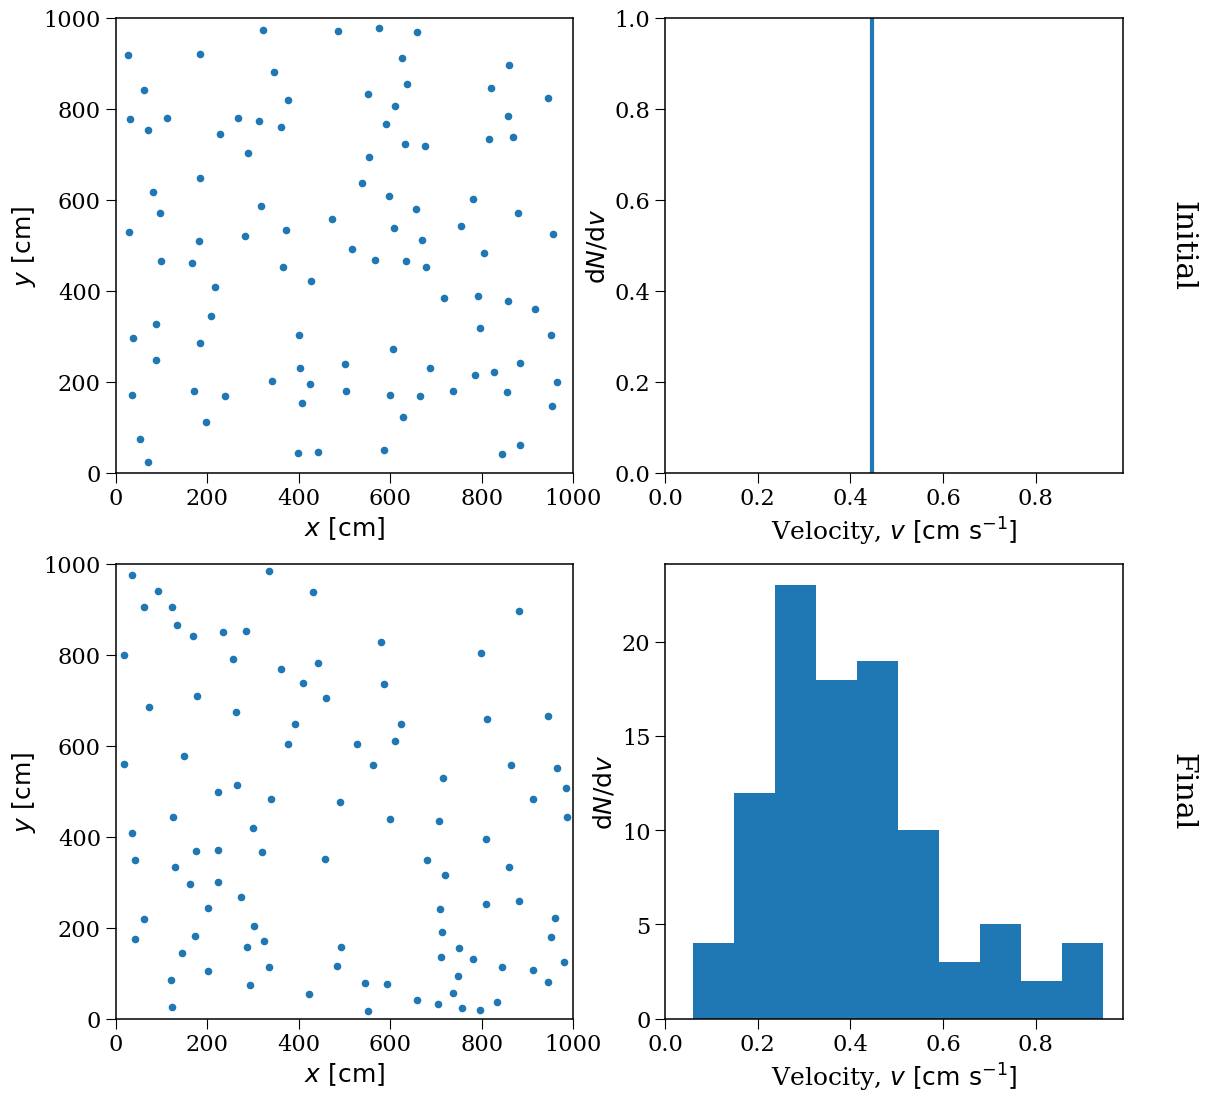
\includegraphics[width=\textwidth]{figures/1b.png}
        \caption{Initial and final distributions of the positions and velocities of the particles. The setting for this simulation were a box of size 1000cm, particles of size 20cm, initial energy of each particle of 0.1 erg and each with a mass of 1g.}
        \label{fig:1b}
    \end{figure}
}

\pagebreak

\question{2a. \textbf{2D Maxwellian}}
\answer{
    Okay let's start with the given function
    \begin{equation}
        f(q, p) \propto \exp \qty( - \frac{E}{k_B T} )
    \end{equation}
    We can first use this to find the speed distribution $\dv{N}{v}$, where $v = \abs{\vb{v}}$.
    \begin{align}
        \dd{N} &= A \exp \qty( - \frac{E}{k_B T} ) \dd{\vb{v}} \\
                  &= A v \exp \qty( - \frac{E}{k_B T} ) \dd{v} \dd{\theta} \\
                  &= A v \exp \qty( - \frac{m v^2}{2 k_B T} ) \dd{v} \dd{\theta}
    \end{align}
    We can normalise this distribution since we know it must be equal to 1 and assume it is isotropic.
    \begin{align}
        \int_0^{\infty} \int_0^{2\pi} A v \exp \qty( - \frac{m v^2}{2 k_B T} ) \dd{v} \dd{\theta} &= 1 \\
        2 \pi A \int_0^{\infty} v \exp \qty( - \frac{m v^2}{2 k_B T} ) \dd{v} &= 1 \\
        2 \pi A \cdot \frac{k_B T}{m} &= 1 \\
        A &= \frac{m}{2 \pi k_B T}
    \end{align}
    This implies that the final distribution (after integrating out the angles) is
    \begin{equation}\label{eq:v_dist}
        \boxed{ \dv{N}{v} = \frac{m v}{k_B T} \exp \qty( - \frac{m v^2}{2 k_B T} ) }
    \end{equation}
    Now I can be lazy and do a change of variables instead of going through that whole rigmarole again since we know that
    \begin{align}
        v &= \qty(\frac{2 E}{m})^{1/2} \\
        \dv{v}{E} &= \qty(\frac{2}{m})^{1/2} \cdot \frac{1}{2} E^{-1/2} \\
                  &= \qty(\frac{1}{2 m E})^{1/2}
    \end{align}
    This means that we can write the energy distribution as
    \begin{align}
        \dv{N}{E} &= \dv{N}{v} \dv{v}{E} \\
                  &= \qty(\frac{1}{2 m E})^{1/2} \frac{m \qty(\frac{2 E}{m})^{1/2}}{k_B T} \exp \qty( - \frac{m \qty(\frac{2 E}{m})}{2 k_B T} ) \\
        \Aboxed{ \dv{N}{E} &= \frac{1}{k_B T} \exp \qty( - \frac{E}{k_B T} ) }\label{eq:e_dist}
    \end{align}
}

\question{2b. \textbf{Show simulation approaches distribution}}
\answer{
    In Figure~\ref{fig:2b}, I show that my simulated speed and energy distributions approaches the distributions given in Equations~\ref{eq:v_dist} and \ref{eq:e_dist}. To make this plot I use a box of 300 particles of radius 3cm and mass 1g, where the box is 750cm in length and each particle starts with 1 erg of energy.
    
    I then evolve the simulation for 10,000 seconds and save the distributions at this point. Next, to increase the number of samples I evolve it 100 more times for 100 seconds each and save the speeds and energies in each of these cases. In this way, I effectively have a sample of 30,000 particles instead of 300 and so the histogram looks nice and smooth (IMHO) :D
    
    One can see that the simulation reproduces the analytic distributions quite nicely, fun!
    \begin{figure}[htb]
        \centering
        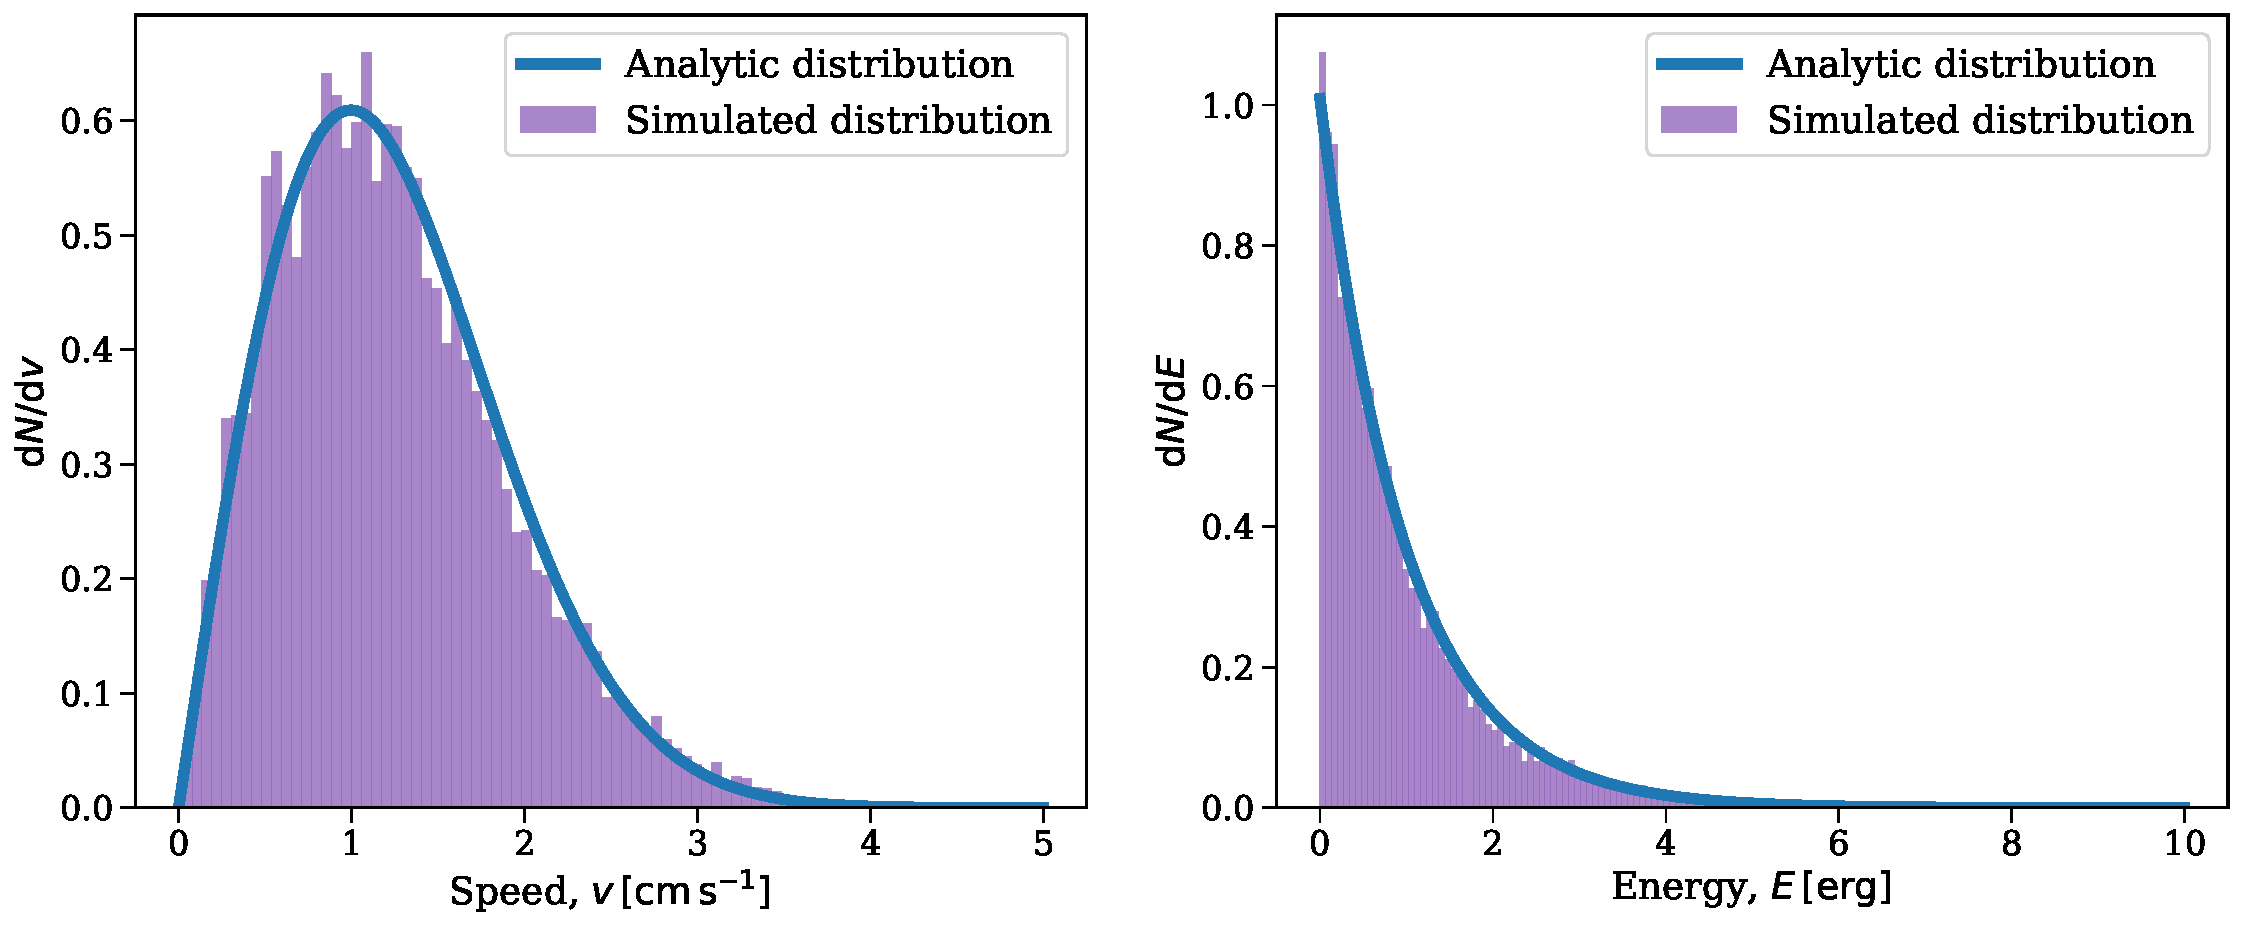
\includegraphics[width=\textwidth]{figures/2b.pdf}
        \caption{Plot showing the speed and energy distributions of the simulation converging to the expected analytic result. For the analytic distributions I use Equations~\ref{eq:v_dist} and \ref{eq:e_dist}.}
        \label{fig:2b}
    \end{figure}
}

\question{2c. \textbf{Multiple masses}}
\answer{
    In Figure~\ref{fig:2c_velocity}, I show the new distributions for when half of the masses are 10 times higher.
    
    Let's talk about the speed distribution first (left side). The distribution no longer follows a single Maxwellian, but instead follows a \textit{mixture} of two Maxwellians. The total distribution is found by summing the distribution using the $v_{\rm rms}$ from the lower mass and higher mass particles separately (and then normalising). This makes sense because the particles of different masses will move at different speeds when given the same kinetic energy and so they form two distributions.
    
    The distribution for the energy is found in the same way. However, the distribution still resembles a single Maxwellian since the functional form doesn't explicitly depend on the mass. It also makes sense intuitively since each particle is given the same initial kinetic energy regardless of mass.
    
    \begin{figure}[htb]
        \centering
        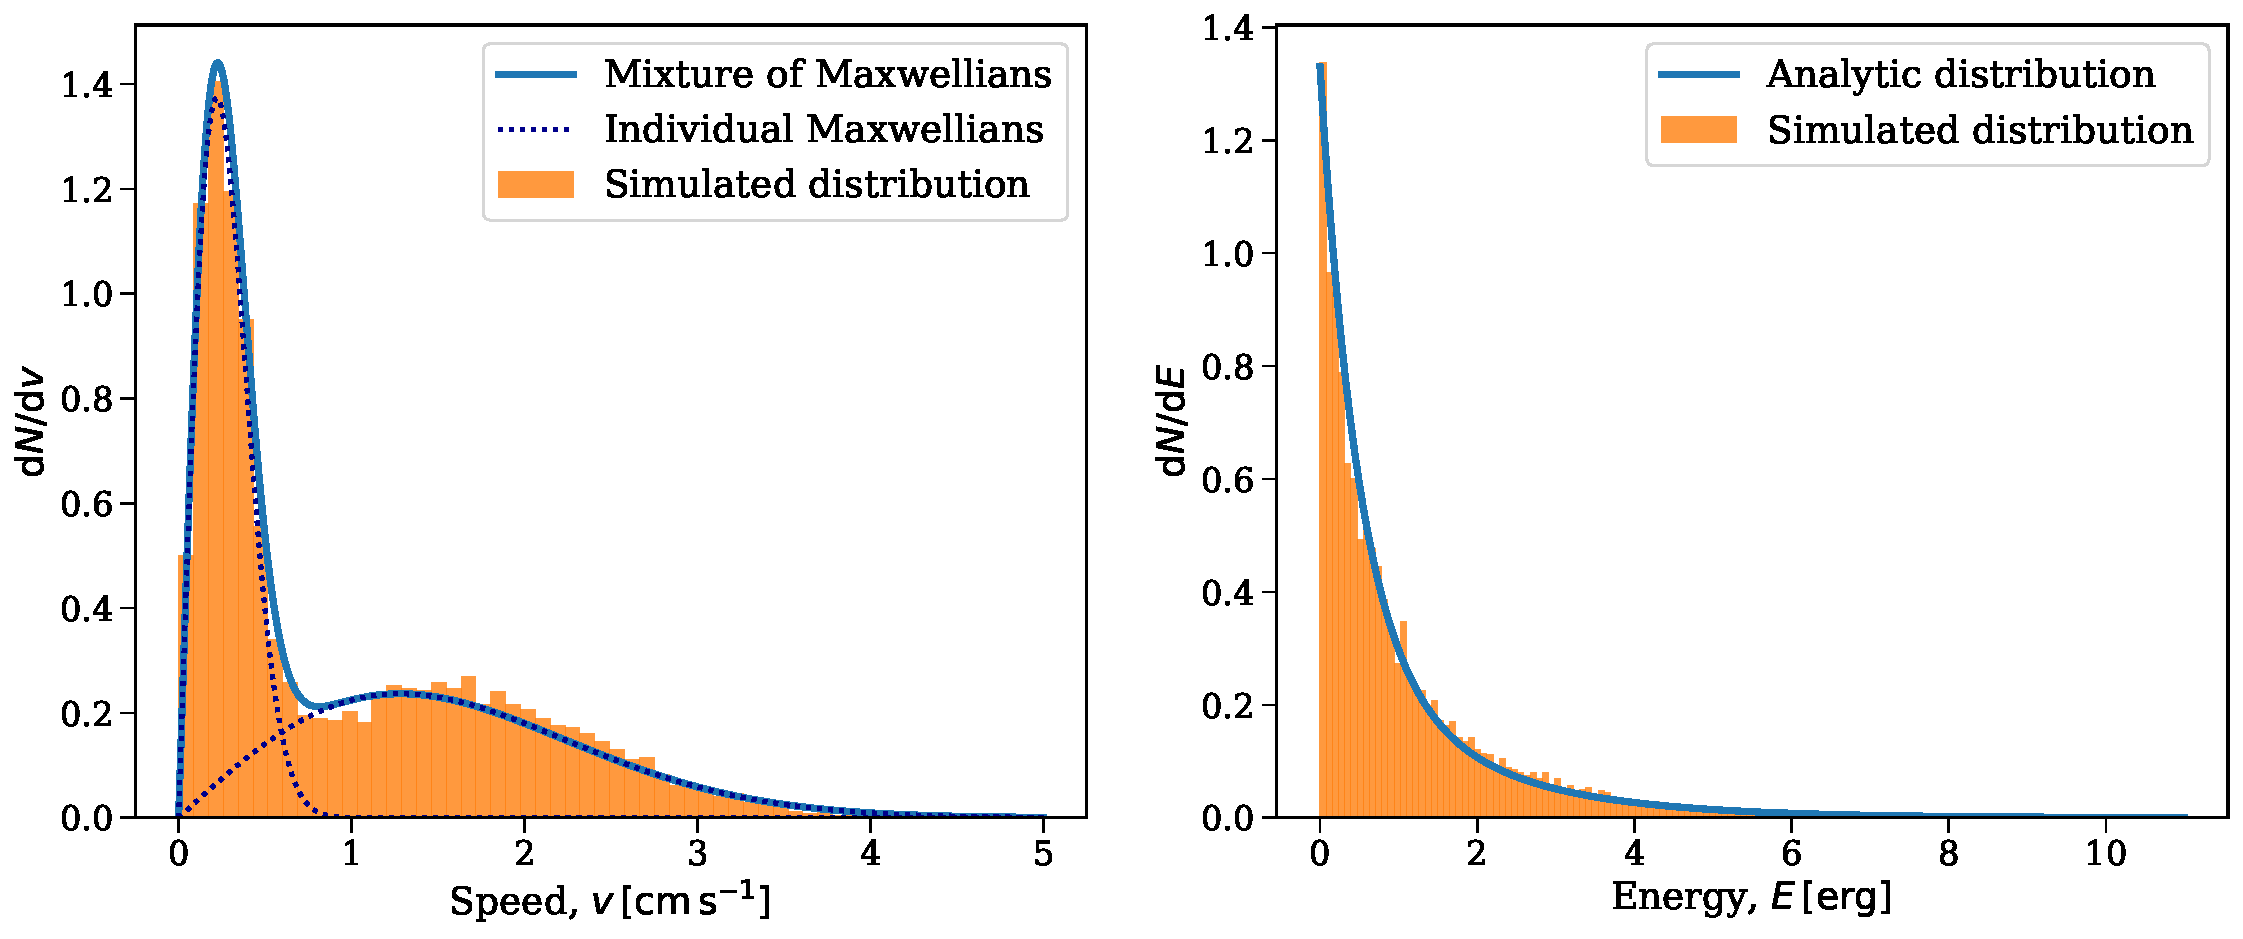
\includegraphics[width=\textwidth]{figures/2c.pdf}
        \caption{As Figure~\ref{fig:2b}, except now half of the particles have masses of 10 g. For the speed distribution I overlay individual Maxwellians for each of the subpopulations as well as their normalised sum.}
        \label{fig:2c_velocity}
    \end{figure}
}

\question{3a. \textbf{Relaxation Criterion}}
\answer{
    For a numerical criterion I used a K-S test on both the speed and the energy. I convert the distributions into CDFs and then used \texttt{scipy.stats.kstest} to attain p-values for both tests. Once both tests attain a p-value of at least 0.05 I assume that the system has relaxed to the steady state.
}

\question{3b. \textbf{Relaxation time derivation}}
\answer{
    The relaxation timescale is essentially the amount of time it takes the system to forget its initial conditions. This loss of information will occur during collisions and thus we can write the relaxation timescale as a function of the number of collisions.
    
    So, let's first derive the average time between collisions for a particle. We are given that the initial speed of the particle is $v_0$, its cross section is $\sigma$ and the number density of particles is $n$. Given these values, we know that the area that the particle moves through in a time $t$ is
    \begin{equation}
        A = \sigma v_0 t.
    \end{equation}
    Then the number of collisions that occurs is this area multiplied by the number of density and it is then trivial to convert this to an average time until a collision.
    \begin{align}
        n_{\rm collision} = n \sigma v_0 t,\\
        t_{\rm one-collision} = \frac{1}{n \sigma v_0}
    \end{align}
    Finally, we can write that the relaxation timescale is the time for $X$ collisions to occur and so it is
    \begin{equation}\label{eq:t_relax}
        \boxed{ \tau_{\rm relax} = \frac{X}{n \sigma v_0} }
    \end{equation}
    Deciding on the exact value of $X$ is a more difficult decision since we would need to know how many collisions every particles needs to have to forget their initial conditions and so for now I simply state that $\tau_{\rm relax}$ scales in this way.
}

\question{3c. \textbf{Comparison with criterion}}
\answer{
    I compare my answers in 3a and 3b in Figure~\ref{fig:3c}. I found that value of $X = 1.2$ gave a reasonably good fit and so I used that in the plots. For the simulations I used the same default values as problem 1 and varied the number of particles and their size.
    
    For each respective number of particles and radius, I ran the simulation 10 times and I plot these results as error bars spanning the full range with a point at the median of the values. You can see that the results approximately agree!
    \begin{figure}
        \centering
        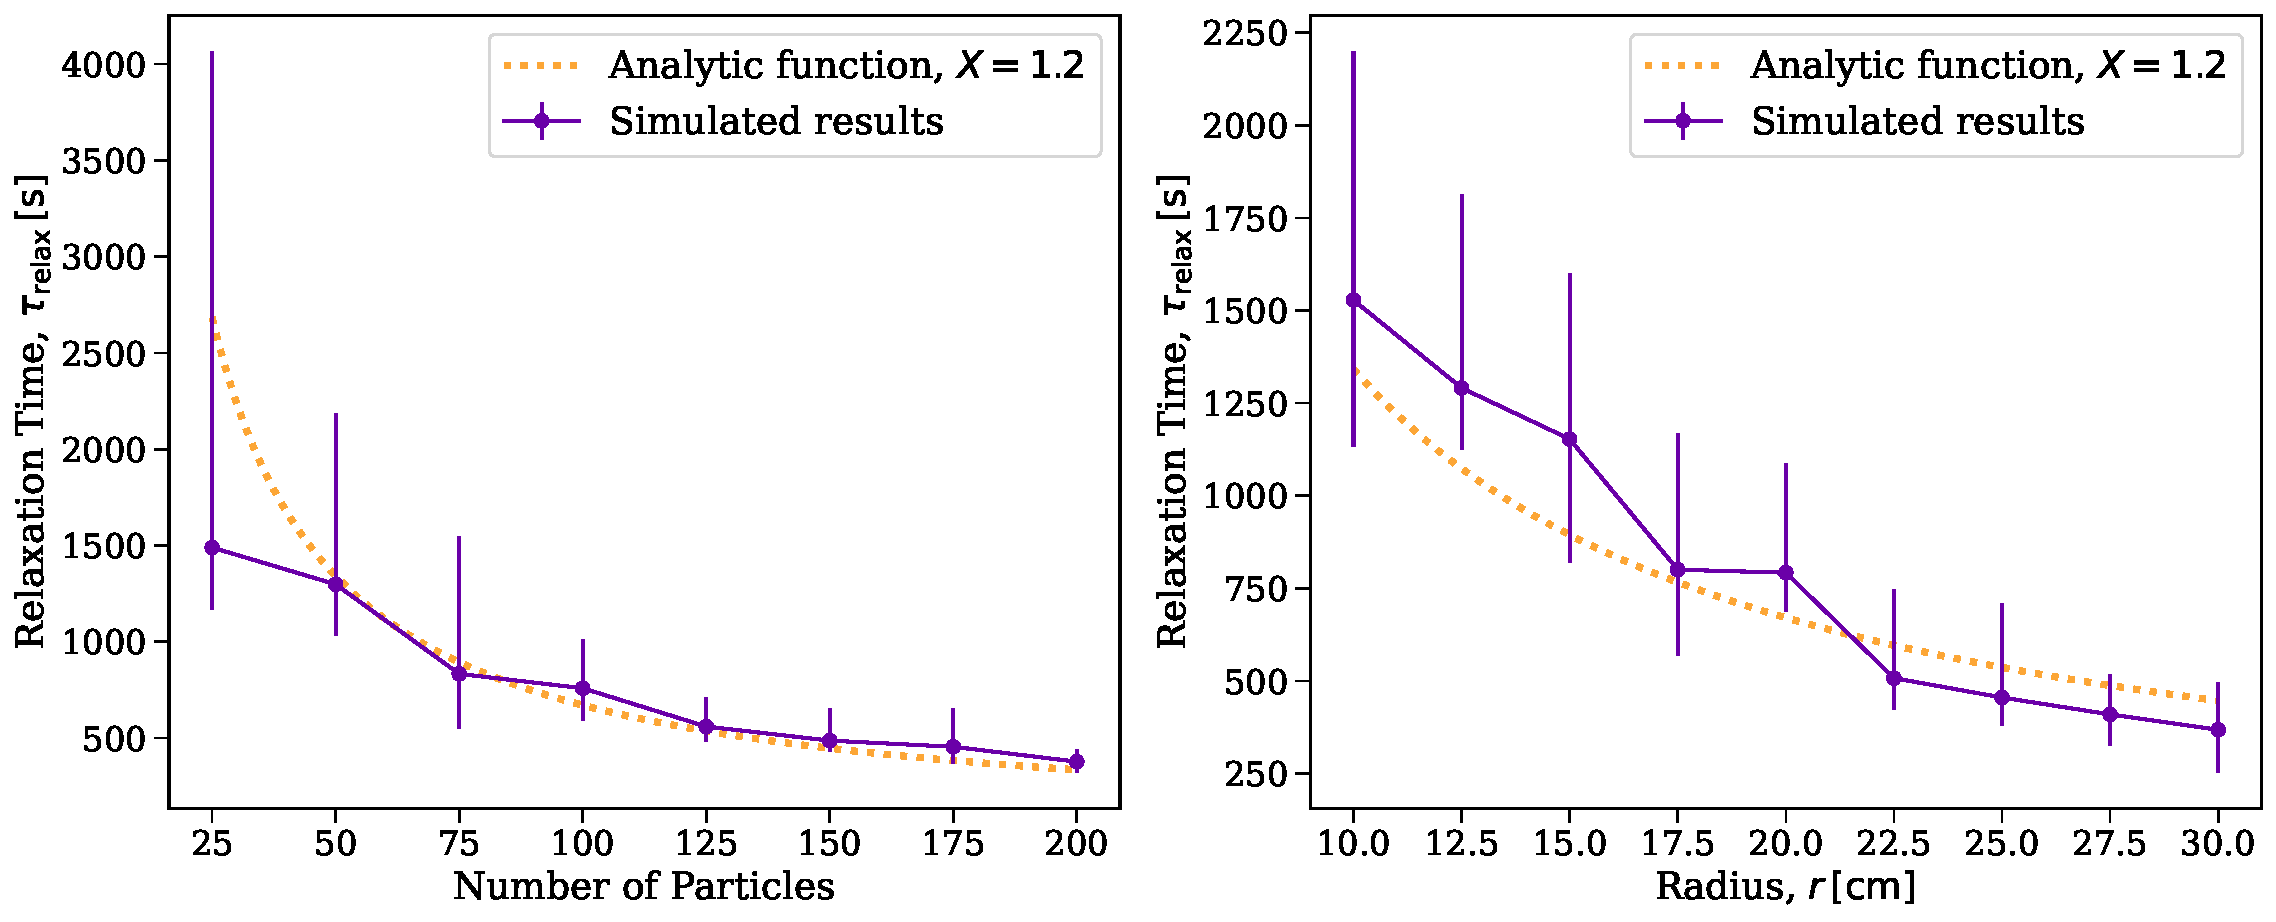
\includegraphics[width=\textwidth]{figures/3c.pdf}
        \caption{A comparison of the numerical criterion from 3a with the analytic formula in 3b. I use a value of $X = 1.2$ in Equation~\ref{eq:t_relax} since that appears to give a reasonable fit.}
        \label{fig:3c}
    \end{figure}
}

\question{\textbf{4. Pressure (Extra Credit)}}
\answer{
    In Figure~\ref{fig:4}, I show that the relation $P = n k_B T$ holds for my simulation. For right-hand side we can write that
    \begin{align}
        n k_B T &= \frac{N}{A} \cdot \frac{1}{2} m v_{\rm rms}^2 \\
                &= \frac{N m v_{\rm rms}^2}{2 L^2}
    \end{align}
    where $N$ is the number of particles, $L$ is the length of one side of the box, $m$ is the mass of particles and $v_{\rm rms}$ is the root-mean-square velocity. Then for the left-hand side we can write that the average pressure on the wall of the box over the whole simulation is simply
    \begin{align}
        P &= \frac{\Delta p}{4 L \cdot \Delta t} \\
          &= \frac{\sum_{i=1}^{N_{\rm collide}} 2 m \abs{v_{\perp, i}}}{4 L \cdot \Delta t}
    \end{align}
    where $N_{\rm collide}$ is the number of collisions with the walls, $v_{\perp}$ is the speed in the direction perpendicular to the wall with which the particle collided and $\Delta t$ is the length of time for which the simulation was run.
    
    You can see from the bottom panel of Figure~\ref{fig:4} that my simulation shows strong agreement between the value for $P$ and $n k_B T$ across many different values of $N$ (and therefore $n$) and thus shows that this relation holds. For reference, I created this figure using a box of size 1000cm and particles with initial KE of 1 erg, masses of 1g and radii 5cm.
    \begin{figure}[htb]
        \centering
        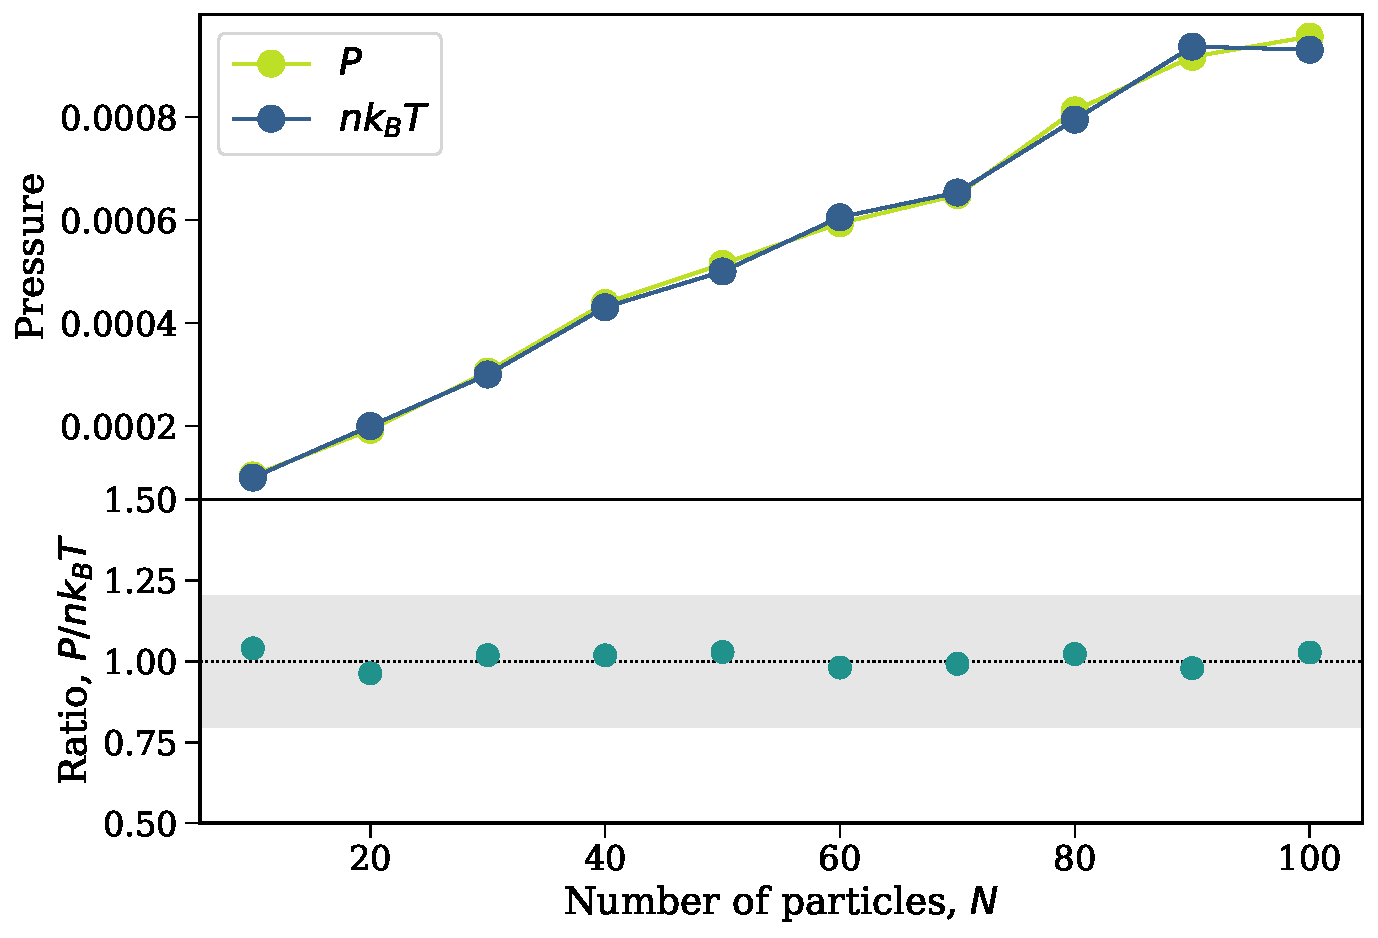
\includegraphics[width=\textwidth]{figures/4.pdf}
        \caption{Demonstration that $P = n k_B T$ holds for my simulation. The top panel plots the values of $P$ and $n k_B T$ separately for different values of $N$. The bottom panel shows their ratio with a line through unity and shading to indicate a 20\% difference.}
        \label{fig:4}
    \end{figure}
}

\end{document}
